\subsubsection{LIRA}

В данном разделе рассматривается фреймворк LIRA (Learning-based Query-aware Partition Framework), предложенный для решения проблем эффективности приближенного поиска ближайших соседей (ANN). Основное внимание уделяется ключевой идее авторов - использованию избыточности хранения (редундантности) для борьбы с неравномерностью распределения данных. \cite{Lyra}

\textbf{Проблема длинного хвоста в распределении ближайших соседей}

Классические методы ANN, основанные на жестком разбиении данных на шарды (hard partitioning), сталкиваются с фундаментальным ограничением, связанным с природой распределения данных в высокоразмерных пространствах. Даже при удачном выборе центроидов кластеров результаты запроса часто рассеяны по множеству шардов. Это явление, получившее название «длинный хвост» (long-tailed distribution), проявляется в том, что несколько соседей могут находиться на одном шарде, в то время как один-два соседа - в нескольких других.

Авторы провели серию экспериментов на реальных данных SIFT, чтобы подтвердить устойчивость этого феномена. Рисунок~\ref{fig:longtail_phenomenon} демонстрирует, что при различном количестве шардов \(B\) (от 8 до 64) тысячи запросов из десяти тысяч имеют распределение, в котором хотя бы один шард содержит ровно одного ближайшего соседа.

\begin{figure}[htbp]
    \centering
    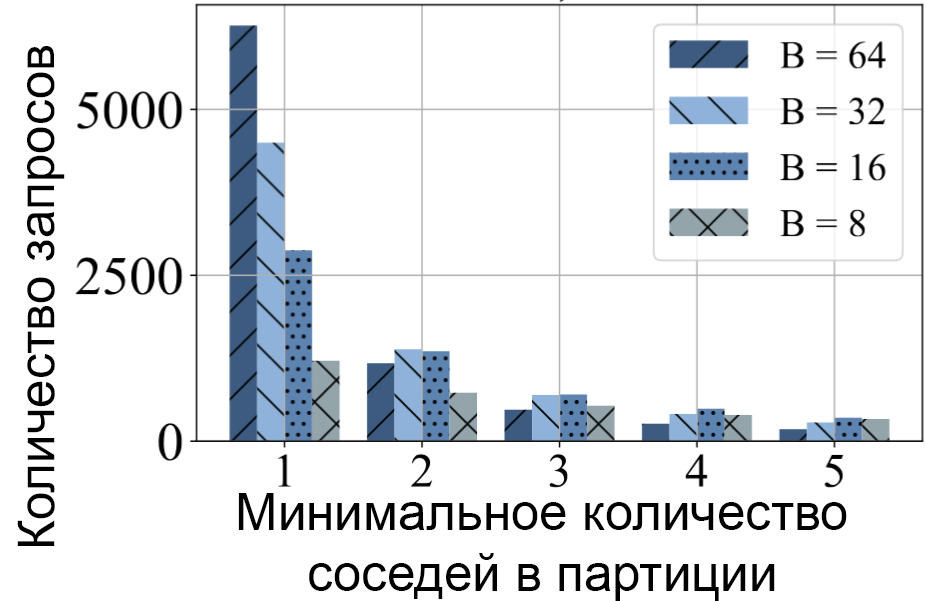
\includegraphics[width=0.6\textwidth]{extras/lyra/longtail.png}
    \caption{Распределение запросов с длиннохвостыми kNN. Значительная часть запросов имеет хотя бы один шард с ровно одним соседом.}
    \label{fig:longtail_phenomenon}
\end{figure}

Этот, казалось бы, незначительный остаток (один вектор в шарде) оказывает непропорционально большое влияние на эффективность поиска. Если не учесть эту редкий шард, полнота поиска упадет. Если учесть - придется тратить ресурсы на просмотр шарда, где находится лишь один полезный результат. Именно для разрешения этой дилеммы и требуется пересмотр самого принципа организации данных.

\textbf{Концепция редундантности}

В ответ на ограничения жесткого разбиения авторы фреймворка LIRA предлагают отказаться от принципа «одна точка - один шард» и ввести элемент избыточности (redundancy) в структуру хранения. Ключевая идея заключается в том, чтобы стратегически дублировать определенные вектора данных, тем самым сглаживая длинный хвост распределения и уменьшая количество шардов, которые необходимо посетить для достижения высокой полноты поиска.

Цель редундантности можно проиллюстрировать простым примером. Пусть распределение kNN для некоторого запроса имеет вид \([5, 4, 1, 0, 0]\), что означает необходимость просмотра трех шардов. Если длиннохвостый вектор из третьего шарда продублировать в одну из двух первых, распределение изменится на \([5, 5, 0, 0, 0]\), и для покрытия всех \(k\) соседей потребуется просмотреть всего два шарда.

Однако реализация этой идеи сталкивается с двумя серьезными вызовами. Первый вызов связан с идентификацией векторов, которые являются длинным хвостом. Прямой подход требует вычисления kNN для всех точек данных, что имеет квадратичную сложность \(O(N^2)\) и неприменим для больших данных. Второй вызов заключается в выборе шарда для дублирования: необходимо определить, в какой именно шард поместить копию вектора, чтобы это максимально сократило будущие запросы.

\textbf{Алгоритм дублирования}

Этап 1: Оценка вероятностей с помощью обученной модели.

Для всех векторов \(v \in \mathcal{D}\) вычисляются предсказания обученной модели \(f\), которая для каждого вектора (рассматриваемого как гипотетический запрос) возвращает вектор вероятностей:
$$
\hat{p}^v = f(v, I_v) = [\hat{p}^v_1, \hat{p}^v_2, \dots, \hat{p}^v_B] \in [0, 1]^B
$$
где \(I_v = [dist(v, c_1), dist(v, c_2), \dots, dist(v, c_B)]\) - расстояния от вектора \(v\) до центроидов всех шардов, а \(\hat{p}^v_b\) интерпретируется как вероятность того, что \(b\)-й шард содержит хотя бы одного из \(k\) ближайших соседей вектора \(v\).

Этап 2: Оценка собственного nprobe для каждого вектора.

Для каждого вектора \(v\) вычисляется его собственное прогнозируемое количество шардов, необходимых для покрытия его \(k\) ближайших соседей:
$$
\hat{n}^*_v = \left|\left\{ b \mid \hat{p}^v_b > \sigma \right\}\right|
$$
где \(\sigma\) - пороговое значение (по умолчанию 0.5). Величина \(\hat{n}^*_v\) является оценкой того, насколько широко распределены ближайшие соседи самого вектора \(v\) по различным шардам.

Этап 3: Выявление длиннохвостых векторов-кандидатов.

Авторами эмпирически обнаружена корреляция: векторы с большим значением \(\hat{n}^*_v\) с высокой вероятностью сами оказываются в длинном хвосте распределения kNN для других запросов. Формально это можно записать как:
$$
P\left(v \in \text{LongTail}(q) \mid \hat{n}^*_v > \tau \right) \gg P\left(v \in \text{LongTail}(q)\right)
$$
где \(\text{LongTail}(q)\) - множество векторов, являющихся единственными представителями своих шардов в результатах запроса \(q\), а \(\tau\) - некоторый порог.

На основе этой корреляции формируется множество кандидатов на дублирование:
$$
\mathcal{D}_{\text{pick}} = \left\{ v \in \mathcal{D} \mid \hat{n}^*_v \geq \text{Percentile}_{\eta}(\{\hat{n}^*_u \mid u \in \mathcal{D}\}) \right\}
$$
где \(\text{Percentile}_{\eta}\) - \(\eta\)-й процентиль распределения \(\hat{n}^*\) по всему множеству данных, а \(\eta\) - гиперпараметр алгоритма (обычно 3-5\%).

Этап 4: Выбор целевого шарда для дублирования.

Для каждого вектора-кандидата \(v \in \mathcal{D}_{\text{pick}}\) необходимо выбрать целевой шард \(b_{\text{target}}(v)\), в которую будет помещена его копия. Выбор основывается на следующем эмпирическом наблюдении: множество реплика-шардов \(R(v)\) (шардов, в которые следует дублировать вектор для максимального сокращения будущих запросов) с высокой точностью покрывается top-M шардов по значению \(\hat{p}^v_b\):
$$
\text{Recall}_{\text{rep}}(M) = \frac{| \text{Top}_M(\hat{p}^v) \cap R(v) |}{|R(v)|} \approx 1 \quad \text{при умеренных } M
$$

На практике используется следующее правило выбора:
$$
b_{\text{target}}(v) = \arg\max_{b \neq b_{\text{orig}}(v)} \hat{p}^v_b
$$
то есть выбирается шард с наибольшей предсказанной вероятностью среди всех шардов, кроме исходной.

В случае, если \(\arg\max_{b} \hat{p}^v_b = b_{\text{orig}}(v)\) (что возможно, хотя исходный шард и имеет наибольшую вероятность), выбирается шард со вторым по величине значением \(\hat{p}^v_b\):
$$
b_{\text{target}}(v) = \arg\max_{b \neq b_{\text{orig}}(v)} \hat{p}^v_b = \underset{b \neq b_{\text{orig}}(v)}{\operatorname{argmax}} \hat{p}^v_b
$$

Этап 5: Дублирование и обновление структуры данных.

Для каждого выбранного вектора \(v \in \mathcal{D}_{\text{pick}}\) создается его копия \(v'\) (полностью идентичный вектор), которая добавляется в целевой шард \(P_{b_{\text{target}}(v)}\):
$$
P_{b_{\text{target}}(v)} \leftarrow P_{b_{\text{target}}(v)} \cup \{v'\}
$$

Исходный вектор \(v\) при этом остается в своём шарде \(P_{b_{\text{orig}}(v)}\). В результате общий объем данных увеличивается на \(|\mathcal{D}_{\text{pick}}|\) векторов, что составляет \(\eta\%\) от исходного размера.

\textbf{Использование обучаемой модели для управления редундантностью}

Для решения задач идентификации длиннохвостых векторов и выбора целевых щардов авторы предлагают использовать обучаемую модель. Обучение производится на подмножестве данных, где для каждого обучающего вектора известно, на каких шардах находятся его истинные ближайшие соседи. Модель учится предсказывать эту информацию для произвольных запросов.

В основе идентификации лежит эмпирически обнаруженная корреляция. Авторы заметили, что вектора с большим собственным \(nprobe^*\) (количеством шардов, необходимых для покрытия их собственных kNN) с высокой вероятностью сами оказываются в длинном хвосте у других запросов. Поскольку вычислить истинный \(nprobe^*\) для всех векторов вычислительно дорого, для его оценки используется предсказание обученной модели. Вектора с наибольшим предсказанным \(nprobe\) отбираются в кандидаты на дублирование.

Для выбора целевого шарда также используется предсказание модели. Анализ показал, что шарды, в которые следует дублировать вектор, с высокой точностью входят в число тех, которым модель присваивает наибольшие вероятности для данного вектора. Таким образом, выбор целевого шарда также делегируется обученной модели.

Алгоритм дублирования для вектора \(v\), исходно принадлежащего шарда \(b_{orig}\), выглядит следующим образом. На основе предсказаний модели все шарды ранжируются по убыванию вероятности того, что они содержат ближайших соседей \(v\). Выбирается шард \(b_{target}\) с наивысшим рангом, такая что \(b_{target} \neq b_{orig}\). Вектор \(v\) дублируется в шард \(b_{target}\). В случае, если наивысший ранг у \(b_{orig}\), выбирается следующая по вероятности шарда.

Введение редундантности изменяет не только структуру хранения, но и сам процесс выполнения запросов. После того как избыточные шарды построены, для входящего запроса \(q\) выполняется следующий двухэтапный процесс.

На первом этапе обученная модель используется для предсказания того, какие шарды с наибольшей вероятностью содержат ближайших соседей запроса. Важно отметить, что благодаря предварительному дублированию длиннохвостых векторов, множество таких шардов оказывается меньше, чем в исходной структуре без редундантности.

На втором этапе поиск выполняется только внутри предсказанных шардов с использованием быстрых внутренних индексов (например, HNSW). Все найденные кандидаты собираются, сортируются по расстоянию до запроса, и из них выбираются \(k\) ближайших.

Таким образом, редундантность работает на опережение: еще на этапе построения индекса структура хранения адаптируется таким образом, чтобы будущие запросы требовали просмотра меньшего количества шардов. Это качественно меняет компромисс между полнотой поиска и количеством просматриваемых данных.
